\section{Начальные распределения для CO$_2-$Ar}
\subsection{Точные формулы для распределений}

Из классической механики известно, что при отделении центра масс в системе <<атом + линейная молекула>> образуются две эффективные частицы, где первая частица движется на расстоянии $l$ и имеет массу $\mu_1=\frac{m_1 m_2}{m_1+m_2}$, а вторая, с массой $\mu_2 = \frac{(m_1+m_2)m_3}{m_1+m_2+m_3}$ движется на расстоянии $R$, где $R$ -- расстояние между центром масс линейной молекулы и атомом, $l$ -- длина линейной молекулы.\\
\\
Тогда для связи векторов в ЛСК и МСК у нас получатся слеующие выражения:
\begin{equation}
\label{eq:relation_mol_lab}
\begin{array}{c}
\bbS \, \dot{\mf{r}}_1 = 
 \Bigg\{ \left( \begin{matrix}
l \cos (\Theta )\dot \Theta\\ 
0\\
-l \sin (\Theta) \dot \Theta
\end{matrix}  \right) + 
\left( \begin{matrix}
l\Omega_y \cos (\Theta) \\ 
-l\Omega_x \cos(\Theta) + l\Omega_z \sin(\Theta)\\
-l\Omega_y \sin(\Theta)
\end{matrix}  \right) \Bigg\}\\
\bbS \, \dot{\mf r}_2 =  \Bigg\{ \left( \begin{matrix}
0\\ 
0\\
\dot R
\end{matrix}  \right) + 
\left( \begin{matrix}
\Omega_y R\\ 
-\Omega_x R\\
0
\end{matrix}  \right) \Bigg\}
\end{array}
\end{equation}
причем $\bbS$ -- ортогональная матрица поворота, например, матрица углов Эйлера. 
Для упрощения дальнейших выкладок тильдой пометим компоненты векторов, получающиеся при действии матрицы $\mathbb{S}$ на вектора скорости в лабораторной системе координат.

\begin{equation}
\label{eq:r_tilde}
\begin{array}{c}
\mathbb{S} \, \dot{\mf{r}}_1 = \bbS \left(\begin{matrix}
\dot{x}_1\\
\dot{y}_1\\
\dot{z}_1
\end{matrix}\right)  =
\left(\begin{matrix}
S_{11}\dot{x}_1 + S_{12}\dot{y}_1 + S_{13}\dot{z}_1 \\
S_{21}\dot{x}_1 + S_{22}\dot{y}_1 + S_{23}\dot{z}_1\\
S_{31}\dot{x}_1 + S_{32}\dot{y}_1 + S_{33}\dot{z}_1
\end{matrix}\right)
=  \left(\begin{matrix}
\tilde{r}_{11}\\
\tilde{r}_{12}\\
\tilde{r}_{13}
\end{matrix}\right)
\\
\bbS \, \dot{\mf{r}}_2 = \mathbb{S}\left(\begin{matrix}
\dot{x}_2\\
\dot{y}_2\\
\dot{z}_2
\end{matrix}\right)  =
\left(\begin{matrix}
S_{11}\dot{x}_2 + S_{12}\dot{y}_2 + S_{13}\dot{z}_2 \\
S_{21}\dot{x}_2 + S_{22}\dot{y}_2 + S_{23}\dot{z}_2\\
S_{31}\dot{x}_2 + S_{32}\dot{y}_2 + S_{33}\dot{z}_2
\end{matrix}\right)= \left(\begin{matrix}
\tilde{r}_{21}\\
\tilde{r}_{22}\\
\tilde{r}_{23}
\end{matrix}\right) 
\end{array}
\end{equation}

\begin{equation}
\mL = \frac{\mu_1}{2}\dot{\mf{r}}_1^2 + \frac{\mu_2}{2}\dot{\mf{r}}_2^2 - U(R,\Theta)
\end{equation}

Запишем (\ref{eq:relation_mol_lab}) в качестве системы уравнений, с учетом (\ref{eq:r_tilde}).

\begin{equation}
\label{eq:system}
\begin{cases}
\tilde{r}_{11} = l \dot{\Theta} \cos \Theta  + l\Omega_y \cos \Theta \\
\tilde{r}_{12} = -l\Omega_x \cos \Theta + l\Omega_z \sin \Theta \\
\tilde{r}_{13} = -l \dot{\Theta} \sin \Theta - l \Omega_y \sin \Theta \\
\tilde{r}_{21} = \Omega_y R\\
\tilde{r}_{22} = -\Omega_x R\\
\tilde{r}_{21} = \dot R
\end{cases}
\end{equation}
Предполагая, что в (\ref{eq:system}) 1-е и 3-е уравнения эквивалентны (в конце документа рассмотрен случай отсутствия этого предположения), найдем выражения для скоростей в МСК, решая данную систему линейных уравнений:
\begin{gather}
\left\{
\begin{aligned}
\dot R &= \tilde{r}_{23}\\
\dot \Theta &= -\frac{1}{l\sin \Theta} \lb \tilde{r}_{13}+\frac{1}{R} \tilde{r}_{21} \, l \sin\Theta  \rb \\
\Omega_x &= -\frac{1}{R}\tilde{r}_{22} \\
\Omega_y &= \frac{1}{R} \tilde{r}_{21} \\
\Omega_z &= \frac{1}{\sin \Theta} \lb \tilde{r}_{12}- \frac{1}{R} \tilde{r}_{22}l\cos \Theta \rb
\end{aligned}
\right.
\end{gather}

Мы не будем приводить здесь вывод, однако несложно показать, что гамильтоновы переменные связаны с лагранжевыми переменными для рассматриваемой системы следующим образом:

\begin{gather}
\left\{
\begin{aligned}
p_R &= \mu_2\dot R\\
p_{\Theta} &= \Omega_yl^2 \mu_1 + l^2 \mu_1 \dot \Theta \\
J_x &= -\mu_1 l^2 \Omega_z \sin \Theta \cos \Theta + \Omega_x \lb \mu_1 l^2 \cos^2 \Theta + \mu_2 R^2 \rb \\
J_y &= \mu_1 l^2 \dot \Theta + \Omega_y \lb \mu_2 R^2 + \mu_1 l^2 \rb \\
J_z &= -l^2 \mu_1 \sin \Theta \lb \Omega_x \cos\Theta - \Omega_z \sin\Theta \rb
\end{aligned}
\right.
\end{gather}

Теперь подставим выражения для скоростей в выражения для импульсов.
\begin{gather}
\left\{
\begin{aligned}
p_R &= \mu_2 \tilde{r}_{23}\\
p_{\Theta} &= -\frac{\mu_1 l}{\sin\Theta}\tilde{r}_{13} \\
J_x &= -\mu_2 R \tilde{r}_{22} - \mu_1 l \tilde{r}_{12} \cos \Theta \\
J_y &= \mu_2 R \tilde{r}_{21} - \frac{\mu_1 l}{\sin \Theta}\tilde{r}_{13} \\
J_z &= \mu_1 l\tilde{r}_{12} \sin \Theta
\end{aligned}
\right.
\end{gather}

Рассмотрим вопрос о распределении компонент векторов $\dot{\mf{r}}_1$ и $\dot{\mf{r}}_2$. 
Представим вектор $\dot{\mf{r}}_1$ в лабораторной системе в сферических координатах $\begin{bmatrix} l, & \phi, & \theta \end{bmatrix}$: 
\begin{gather}
\dot{\mf{r}}_1 = \frac{d}{dt}
\begin{bmatrix}
l \sin \theta \cos \phi\\
l \sin \theta \sin \phi\\
l\cos \theta
\end{bmatrix}
=
\begin{bmatrix} 
l \dot{\theta} \cos\theta \cos\phi  - l \dot{\phi} \cos\theta \sin\phi \\ 
l \dot{\theta} \cos\theta \sin\phi + l \dot{\phi} \sin\theta \cos\phi \\ 
 -l \dot{\theta} \sin \theta 
\end{bmatrix} \notag 
\end{gather}

Нетрудно видеть, что вектора $\dot{\boldsymbol{\theta}}$ и $\dot{\boldsymbol{\phi}} \sin \phi$ направлены перпендикулярно оси вращения линейной молекулы, а значит, являются угловыми скоростями вращения линейной молекулы, поэтому распределены как $\mathcal{N}(0,kT/I)$, где $I$ -- момент инерции линейной молекулы. \par
Ради интереса отметим, что будет, если в системе (\ref{eq:system}) не считать 1-е и 3-е уравнения эквивалентными. Для этого умножим первое уравнение на $\sin\Theta$, а второе на $\cos\Theta$, после этого получим
\[
\sin\Theta \: \tilde{r}_{11} + \cos\Theta \: \tilde{r}_{13} = 0
\]
\[
\cot\Theta = -\frac{\tilde{r}_{13}}{\tilde{r}_{11}}
\]
Если $\tilde{r}_{11}$ и $\tilde{r}_{13}$ нормально распределенные случайные величины, то $\cot\Theta$ имеет распределение Коши. \par
Заметим, что алгоритм MH для получения начальных условий может быть применен как только имеется процедура расчета гамильтониана в произвольной точке фазового пространства. Распределения для $\Theta$, $p_R$, $p_T$, $J_x$, $J_y$, $J_z$, полученные по точным формулам и при помощи алгоритма MH, представлены на рис. $\ref{fig:co2ar_comparison}$. Распределение угла $\Theta$ (как угла между двумя равномерно на сфере распределенными векторами) имеет плотность вероятности $f(x) = \displaystyle \frac{1}{2} \sin x$ (на рисунке представлено пунктирной линией), это показано в приложении \ref{app4}.



\begin{figure}[ht!]
	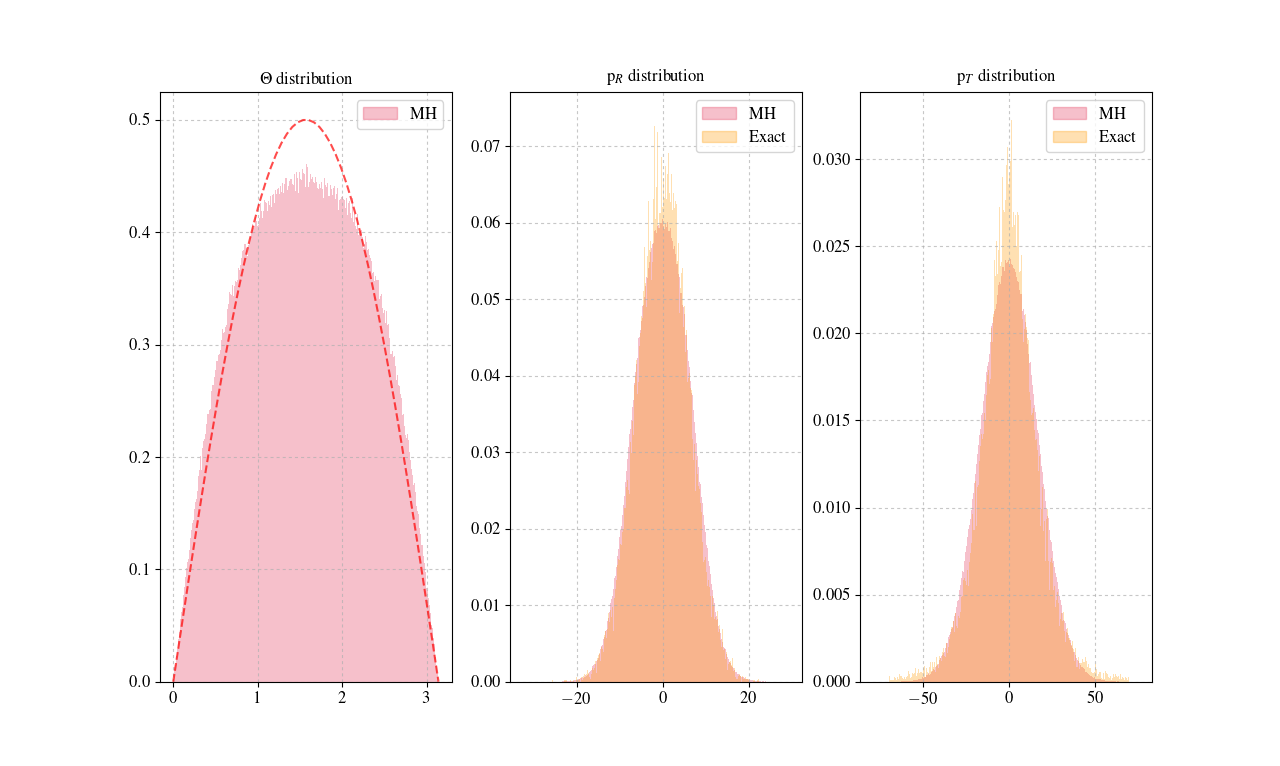
\includegraphics[width=\textwidth]{../pictures/co2arDistributions1.png}
	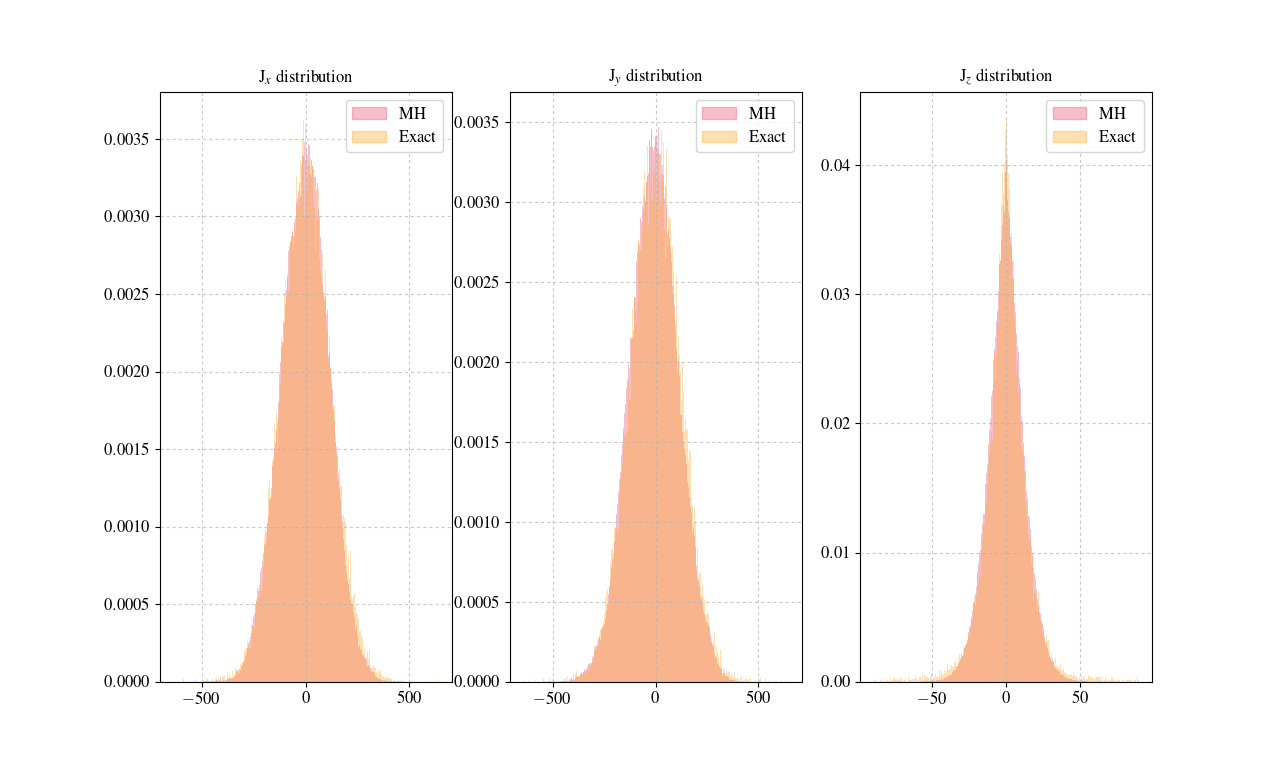
\includegraphics[width=\textwidth]{../pictures/co2arDistributions2.png}
	\caption{Распределения переменных $\Theta$, $p_R$, $p_T$ (\textbf{первый ряд}), $J_x$, $J_y$, $J_z$ (\textbf{второй ряд}) для CO$_2-$Ar при $T = 300 K$, полученные методом $MH$ и по точным формулам, 500.000 точек, $R$ = 20 бор.}
	\label{fig:co2ar_comparison}
\end{figure}


